% Appendix 2
\chapter{پروتکل SAFA }

یکی از پروتکل‌هایی که قابلیت پیاده‌سازی برای فرآیند یادگیری فدرال دارد، پروتکل SAFA است. همان‌طور که در شکل \ref{SAFA} مشهود است، این پروتکل با دسته‌بندی کارگران به ۳ دسته انتخاب شده\LTRfootnote{Picked Client}، تعیین نشده\LTRfootnote{Undrafted Client} و قطع شده\LTRfootnote{Crashed Client} تقسیم می‌کند. این دسته بندی با توجه به نحوه برقراری ارتباط با کارگر در دورهای قبلی هست که در کش ذخیره می‌شود. پروتکل SAFA با استفاده از یک الگوریتم تصادفی، تعدادی از کارگران را به عنوان انتخاب شده انتخاب می‌کند و به آن‌ها دستور می‌دهد که مدل خود را به سرور ارسال کنند. سپس، سرور با دریافت مدل‌های ارسال شده، آن‌ها را با هم ترکیب می‌کند و مدل جدید را به کارگران انتخاب شده برمی‌گرداند. در صورتی که یک کارگر در یک دوره از ارسال یا دریافت مدل عقب بماند، به عنوان قطع شده در نظر گرفته می‌شود و در دوره‌های بعدی حذف می‌شود. همچنین، در صورتی که یک کارگر به طور مکرر در دوره‌های مختلف انتخاب نشود، به عنوان تعیین نشده شناخته می‌شود و احتمال انتخاب آن در دوره‌های آینده کاهش می‌یابد. پروتکل SAFA با استفاده از این روش، سعی دارد تا تعادل بین سرعت و دقت فرآیند یادگیری فدرال را حفظ کند\cite{SAFA}.


\begin{figure}[H]
    \centering
   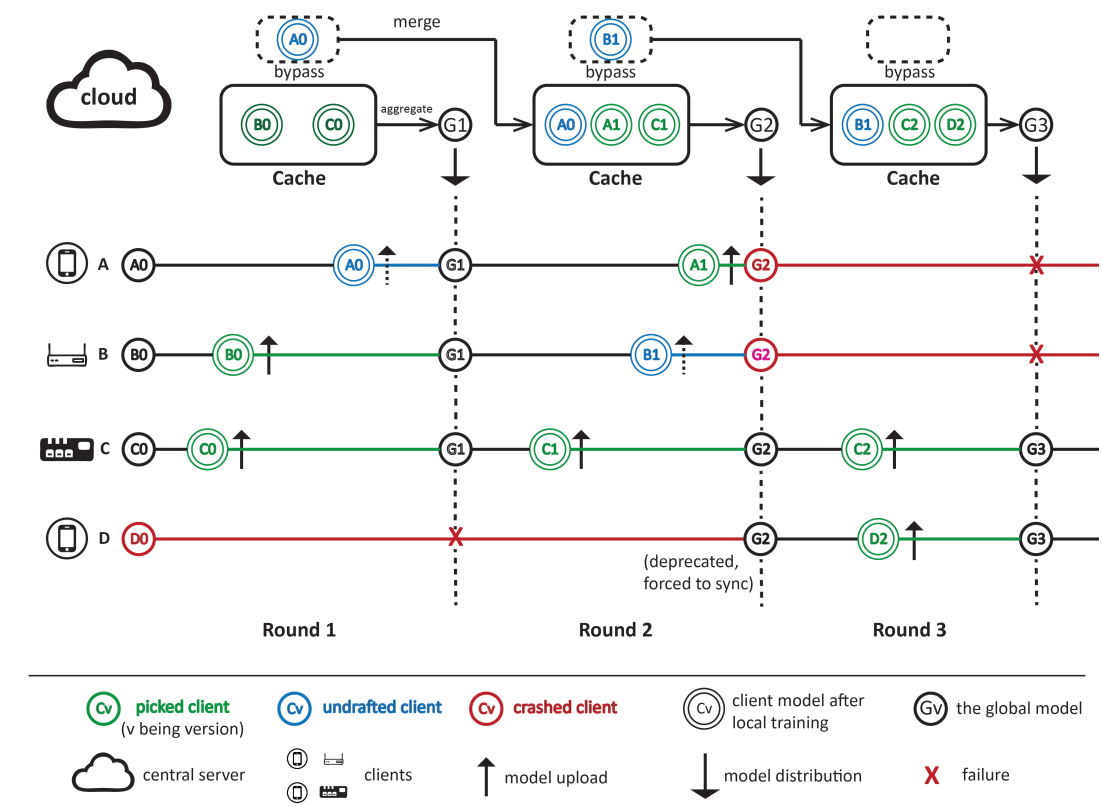
\includegraphics[height=12cm,width=14cm]{./SAFA/ex.png}
   \caption[سناریو‌ای از اجرای پروتکل SAFA در ۳ دور]{ سناریو‌ای از اجرای پروتکل SAFA در ۳ دور\cite{SAFA} }
   \label{SAFA}
   \centering
\end{figure}

با توجه به شکل، کش مدل‌های محلی آخرین کارگر‌های انتخاب شده را که برای تجمیع استفاده می‌شوند، نگه می‌دارد. کارگر‌هایی که نتایج آن‌ها انتخاب نشده‌اند، کارگر‌های رد شده هستند (با رنگ آبی)، مثلاً کارگر A در دور 1 و کارگر B در دور 2.به‌روزرسانی‌های این کارگر‌ها در ساختار میان‌بر\LTRfootnote{Bypass} ذخیره می‌شوند تا از کار بیهوده در سمت محلی جلوگیری شود. کارگر‌هایی که به هر دلیلی (مثل خروج از برنامه یا قطع شدن اینترنت) نمی‌توانند آموزش محلی خود را تکمیل کنند، کارگر‌های خراب هستند (با رنگ قرمز برجسته شده)، مثلاً کارگر D در دور 1. کارگر‌هایی که به‌روزرسانی‌های آن‌ها انتخاب شده‌اند، کارگر‌های انتخاب شده نامیده می‌شوند (با رنگ سبز)، مثلاً کارگر B و C در دور 1.


توزیع مدل با تحمل تأخیر\LTRfootnote{Model Distribution With Lag Tolerance}: در این مرحله، سرور مدل خود را به کارگران مختلف ارسال می‌کند و از آن‌ها می‌خواهد که بر روی داده‌های خود به روزرسانی مدل را انجام دهند. سرور همچنین یک حداکثر زمان تأخیر را برای دریافت مدل‌های به روز شده تعیین می‌کند. این روش اجازه می‌دهد که کارگران با سرعت‌های مختلف و با تأخیرهای متفاوت در فرآیند یادگیری شرکت کنند.

اولین رسیدن برابر است با اولین ادغام\LTRfootnote{First Come First Merge}: در این مرحله، سرور با دریافت مدل‌های به روز شده از کارگران، آن‌ها را با هم ترکیب می‌کند. سرور برای ترکیب کردن مدل‌ها، از الگوریتم «اولین رسید، اولین ترکیب شد» استفاده می‌کند. این الگوریتم به این صورت است که سرور همواره یک نسخه از مدل را نگه دارد و هر گاه یک مدل جدید از یک کارگر دریافت کند، آن را با نسخه فعلی ترکیب کرده و نسخه جدید را ذخیره می‌کند.

تجمیع تمایزدهنده\LTRfootnote{Discriminative Aggregation}: در این مرحله، سرور با استفاده از یک الگوریتم تجمیع تمایزدهنده، مقادیر وزن‌های مختلف در مدل را با هم مقایسه کرده و آن‌ها را به صورت چند جمله‌ای درجه دو نمایش می‌دهد. سپس، با استفاده از چند جمله‌ای حاصل، سطح خطای هر وزن را برآورد کرده و وزن‌های با خطای بالاتر را حذف یا کم کاربرد می‌کند. این روش باعث بهبود دقت و کارآمدی فرآیند یادگیری فدرال می‌شود.

باتوجه به کاربرد‌های متنوع این پروتکل و قابلیت انعطاف بالا خصوصاً زمانی که دستگاه‌های کارگر از سخت‌افزارهای ناهمگون بهره ببرند می‌تواند به‌شدت فرآیند یادگیری را تسریع کند.

